\documentclass[10pt]{exam}
\usepackage[hon]{template-for-exam}
\usepackage{multicol,tikz}
\usetikzlibrary{shadings,decorations.pathmorphing,arrows.meta}

\title{Honors Physics Equation Sheet (Fall Final Exam)}
\author{Rohrbach}
\date{\today}

\begin{document}
\maketitle

\section*{Basic Kinematics}

\begin{align*}
  \bar{v} &\equiv \frac{\Delta x}{\Delta t} &
  \bar{a} &\equiv \frac{\Delta v}{\Delta t} &
  \bar{v} &= \frac{v+v_0}{2}
\end{align*}


\section*{Kinematic Equations}

\vspace{-3em}

\begin{multicols}{3}
  \begin{center}
  
      \begin{align*}
        v = v_0 + a t
      \end{align*}
      ``Old Faithful''
    
      \begin{align*}
        x = x_0 + v_0t + \frac{1}{2}at^2
      \end{align*}
      ``Big Chalupa''
    
      \begin{align*}
        v^2 = v_0^2 + 2a \left( x - x_0 \right)
      \end{align*}
      ``Ain't Got No Time''
  \end{center}
\end{multicols}


\section*{Range Equation}

\begin{align*}
  R &= \frac{v_0^2 \sin\left(2\theta\right)}{g}
\end{align*}

\section*{Vectors \& Trig}

\begin{minipage}{4in}
  \begin{center}
    \begin{align*}
      \sin{\theta} & =\frac{\text{opp}}{\text{hyp}} &
      \cos{\theta} & =\frac{\text{adj}}{\text{hyp}} &
      \tan{\theta} & =\frac{\text{opp}}{\text{adj}}
    \end{align*}
  \end{center}
\end{minipage}
%
\begin{minipage}{2in}
  \begin{center}
    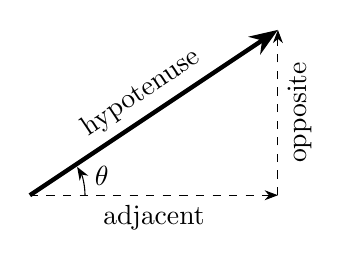
\begin{tikzpicture}[
      every node/.append style={},
      component/.append style={
        dashed,
        -{Stealth}
      },
      resultant/.append style={
        ultra thick,
        -{Stealth}
      },
      scale=0.7
  ]
    \draw[resultant] 
              (0,0) -- (4.5,3) 
                node[midway,anchor=south,rotate=33.7]{hypotenuse};
    \draw[component] 
              (0,0) 
              -- (4.5,0) 
                node[midway,anchor=north]{adjacent} ;
    \draw[component] 
              (4.5,0)
              -- (4.5,3) 
                node[midway,anchor=north,rotate=90]{opposite} ;
    \draw[-Stealth] (1,0) node[anchor=south west]{$\theta$}
              arc[
                start angle = 0,
                end angle = 31, 
                radius = 1
              ];
  \end{tikzpicture}


  \end{center}
\end{minipage}


\section*{Forces}

\begin{align*}
  \Sigma F &= ma &
  F_G      &= mg &
  F_{f,s}  &= \mu_s F_N &
  F_{f,k}  &= \mu_k F_N
\end{align*}

\section*{Circular Motion \& Gravitation}

\begin{align*}
  \Sigma F_C &= ma_C = \frac{mv^2}{r} &
  a_C        &= \frac{v^2}{r} &
  F_G        &= \frac{G m_1 m_2}{r^2} \\
  &&&& G     &= 
        \SI{6.67e-11}{\newton \meter^2\per\kilo\gram^2}
\end{align*}

\section*{Work \& Energy}

\begin{align*}
  W    &= F_\parallel d &
  KE   &= \frac{1}{2} mv^2 &
  PE_g &= mgy &
  PE_e &= \frac{1}{2} kx^2
\end{align*}

\begin{align*}
  W &= \Delta KE &
  \Sigma E_0 + W_{NC} &= \Sigma E &
  P &= \frac{W}{t}
\end{align*}



\end{document}